\section{Guidance：如何根据提示词生成}

前面几章讨论的生成模型大多是无条件的：模型从简单分布
$p_{\mathrm{init}}$ 出发，最终生成服从数据分布 $\data$ 的样本。
但实际应用中，我们通常不只是想生成“任意一张图像”或“任意一个对象”，
而是希望生成满足某个条件的信息。例如，给定文本提示词
$y=$“一只柯基犬在雪地里奔跑”，模型应当生成与该提示词匹配的图像。

从概率角度看，这意味着我们的目标从采样
\begin{equation}
  z\sim \data
\end{equation}
变成采样条件分布
\begin{equation}
  z\sim \data(\cdot|y).
\end{equation}
这里 $y$ 可以是文本提示词、类别标签、语音条件、图像条件等。为了避免和前面
“条件概率路径” $p_t(\cdot|z)$ 中的“条件”混淆，本章把对 $y$ 的条件生成称为
\emph{guided generation}。

\subsection{Vanilla Guidance}

最直接的 guided generation 方法是：在训练和采样时都把提示变量 $y$ 输入网络。
设提示变量 $y$ 属于某个空间 $\mathcal{Y}$。例如，若 $y$ 是文本提示词，
$\mathcal{Y}$ 就是文本空间；若 $y$ 是类别标签，$\mathcal{Y}$ 就是离散类别集合。

我们可以把 guided diffusion model 写成
\begin{equation}
  u^\theta:\R^d\times\mathcal{Y}\times[0,1]\to\R^d,
  \qquad
  (x,y,t)\mapsto u_t^\theta(x|y),
\end{equation}
并给定一个 diffusion coefficient
\begin{equation}
  \sigma_t:[0,1]\to[0,\infty).
\end{equation}
对于固定的提示变量 $y$，采样过程为
\begin{equation}
  X_0\sim p_{\mathrm{init}},
  \qquad
  \dd X_t=u_t^\theta(X_t|y)\,\dd t+\sigma_t\,\dd W_t,
  \qquad
  X_1\sim \data(\cdot|y).
\end{equation}
当 $\sigma_t=0$ 时，这就是 guided flow model。

为了简化讨论，本章主要以 flow matching 为例；相同思想可以直接推广到 diffusion
model。若固定某个 $y$，我们可以把数据分布看成 $\data(\cdot|y)$，
于是又回到了无条件生成问题。对应的 guided conditional flow matching 目标为
\begin{equation}
  \mathcal{L}^{\mathrm{guided}}_{\mathrm{CFM}}(\theta)
  =
  \E_{(z,y)\sim\data(z,y),\,t\sim\mathrm{Unif}[0,1],\,x\sim p_t(\cdot|z)}
  \left[
    \left\|
    u_t^\theta(x|y)-u_t^{\mathrm{target}}(x|z)
    \right\|^2
  \right].
\end{equation}
和无条件 CFM 的差别在于，数据集现在提供的是成对样本 $(z,y)$，而不只是数据
样本 $z$。在实现中，dataloader 需要同时返回图像或视频等数据 $z$ 以及对应的
提示变量 $y$。

\subsection{Classifier Guidance}

理论上，vanilla guidance 已经是在学习条件分布 $\data(\cdot|y)$。但实践中，
仅仅把 $y$ 输入网络往往不够：生成结果可能和提示词不够匹配。原因可能是模型欠拟合、
数据标注噪声较大，或者文本-图像配对本身不够准确。为增强样本对 $y$ 的遵循程度，
人们引入了 guidance scale。

\begin{figure}[htbp]
  \centering
  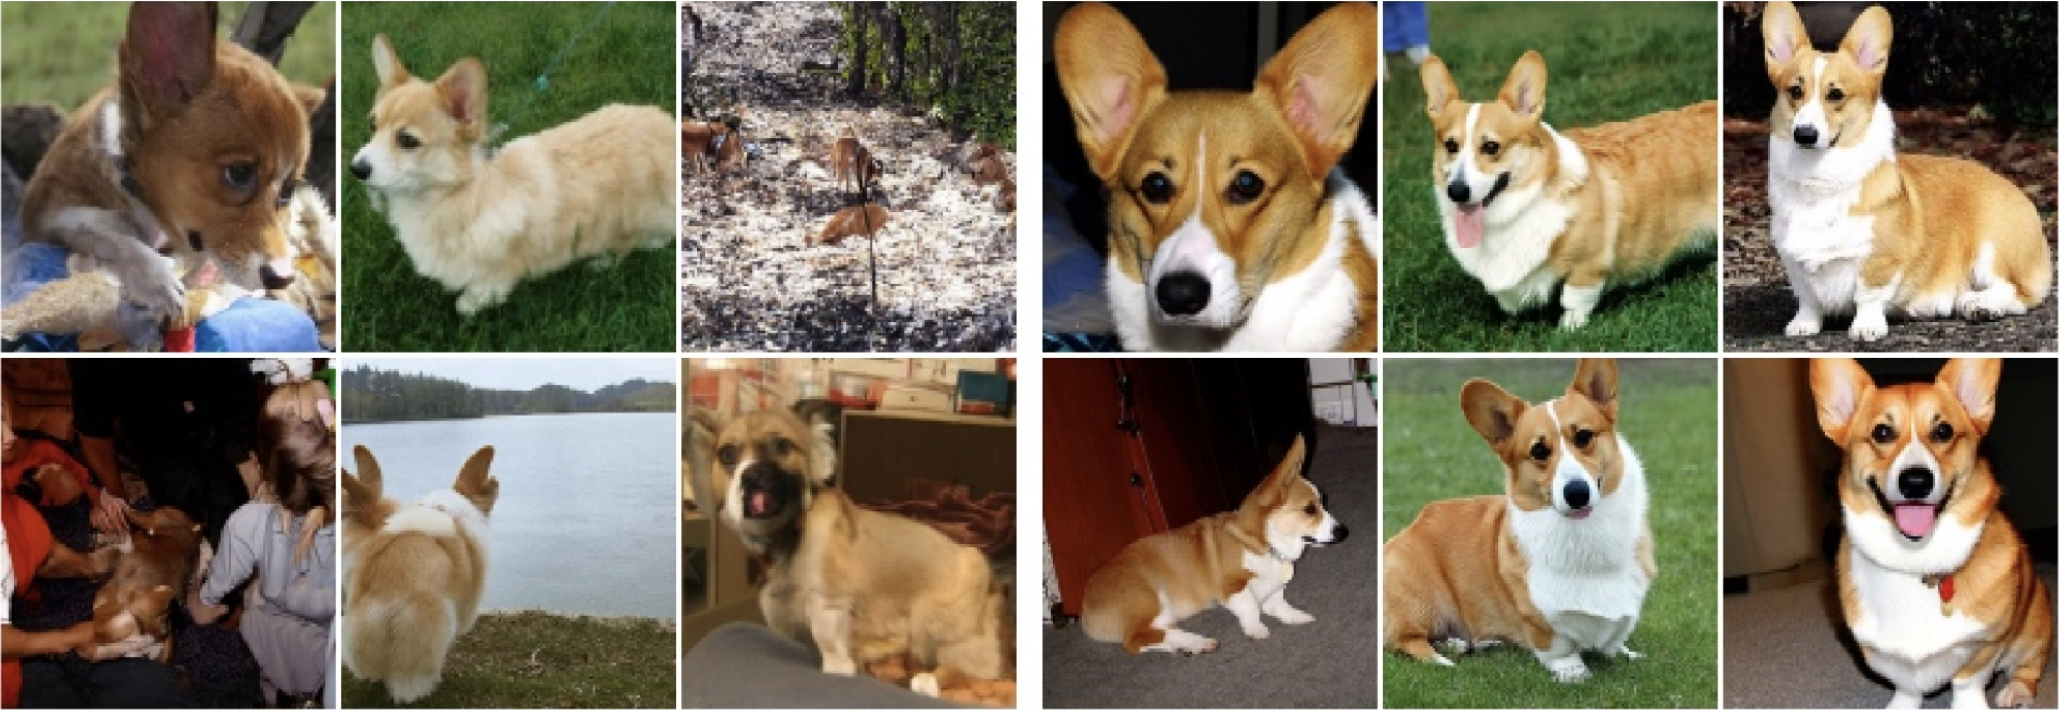
\includegraphics[width=0.9\linewidth]{tex/figures/selected/figure11-corgi-guidance.png}
  \caption{Guidance 可以提高生成结果对提示变量的遵循程度。左侧为 vanilla guidance，右侧为增强 guidance 后的样本。}
  \label{fig:corgi-guidance}
\end{figure}

图~\ref{fig:corgi-guidance} 给出了 guidance 的经验动机：更强的引导通常会带来更好的条件对齐。

先考虑 Gaussian 概率路径。由第四章的转换公式，guided marginal vector field 可以写成
\begin{equation}
  u_t^{\mathrm{target}}(x|y)
  =
  a_t\nabla_x\log p_t(x|y)+b_t x.
\end{equation}
另一方面，由 Bayes 公式，
\begin{equation}
  p_t(x|y)=\frac{p_t(x)p_t(y|x)}{p_t(y)}.
\end{equation}
由于梯度是对 $x$ 求的，$\nabla_x\log p_t(y)=0$，所以
\begin{equation}
  \nabla_x\log p_t(x|y)
  =
  \nabla_x\log p_t(x)
  +
  \nabla_x\log p_t(y|x).
\end{equation}
代入 guided vector field，得到
\begin{equation}
\begin{aligned}
  u_t^{\mathrm{target}}(x|y)
  &=
  b_t x+a_t\left(\nabla_x\log p_t(x)+\nabla_x\log p_t(y|x)\right) \\
  &=
  u_t^{\mathrm{target}}(x)+a_t\nabla_x\log p_t(y|x).
\end{aligned}
\end{equation}
这个式子说明：guided vector field 可以分解为无条件向量场
$u_t^{\mathrm{target}}(x)$ 加上一个“让样本更像提示变量 $y$”的分类器梯度项。

为了强化提示变量的作用，可以把分类器梯度项放大：
\begin{equation}
  \widetilde{u}_t(x|y)
  =
  u_t^{\mathrm{target}}(x)
  +
  w a_t\nabla_x\log p_t(y|x),
  \qquad
  w>1.
\end{equation}
这里 $w$ 称为 guidance scale。若显式训练一个分类器来估计
$\log p_t(y|x)$，再用它的梯度做引导，就得到 classifier guidance。
不过这种方法需要额外训练一个分类器；当 $y$ 是文本这类高维条件时，
学习 $p_t(y|x)$ 也很困难。因此实际大模型中更常用的是 classifier-free guidance。

\subsection{Classifier-Free Guidance}

Classifier-free guidance 的目标是获得与 classifier guidance 类似的强化效果，
但不额外训练分类器。仍从上面的分解出发：
\begin{equation}
  \nabla_x\log p_t(x|y)
  =
  \nabla_x\log p_t(x)+\nabla_x\log p_t(y|x).
\end{equation}
于是
\begin{equation}
\begin{aligned}
  \widetilde{u}_t(x|y)
  &=
  u_t^{\mathrm{target}}(x)
  +
  w a_t\nabla_x\log p_t(y|x) \\
  &=
  u_t^{\mathrm{target}}(x)
  +
  w a_t\left(\nabla_x\log p_t(x|y)-\nabla_x\log p_t(x)\right) \\
  &=
  (1-w)u_t^{\mathrm{target}}(x)+wu_t^{\mathrm{target}}(x|y).
\end{aligned}
\end{equation}
也就是说，强化后的 guided vector field 可以写成无条件向量场和有条件向量场的
线性组合。

为了用一个网络同时表示这两者，我们引入一个特殊空条件 $\emptyset$，表示“不使用
提示变量”。于是可把
\begin{equation}
  u_t^{\mathrm{target}}(x)
  =
  u_t^{\mathrm{target}}(x|\emptyset)
\end{equation}
看成同一个条件模型在空提示下的输出。采样时使用
\begin{equation}
  \widetilde{u}_t^\theta(x|y)
  =
  (1-w)u_t^\theta(x|\emptyset)+wu_t^\theta(x|y).
\end{equation}
当 $w=1$ 时，退化为 vanilla guidance；当 $w>1$ 时，提示变量的影响被放大。
需要注意的是，$w>1$ 时这个向量场通常不再对应真实的
$\data(\cdot|y)$，因此 CFG 本质上是一个经验上非常有效的启发式方法。

\begin{figure}[htbp]
  \centering
  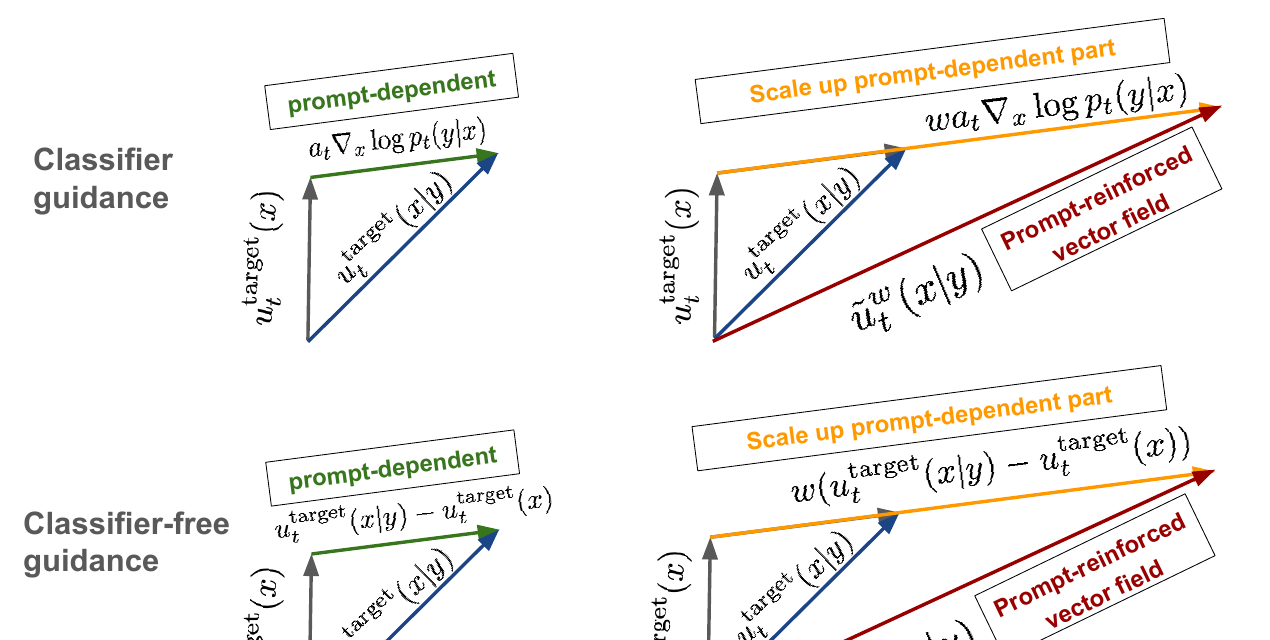
\includegraphics[width=0.95\linewidth]{tex/figures/selected/figure12-cfg-diagram.png}
  \caption{Classifier guidance 与 classifier-free guidance 的几何解释。二者都可以理解为放大 prompt-dependent part，从而得到 prompt-reinforced vector field。}
  \label{fig:cfg-diagram}
\end{figure}

图~\ref{fig:cfg-diagram} 展示了 CFG 的核心直觉：不显式训练分类器，而是用有条件和无条件向量场的差来近似并放大提示相关方向。

\begin{remark}[一般概率路径下的 CFG]
上面的推导用 Gaussian 概率路径解释了 CFG 的直觉，特别是“放大一个隐式分类器
梯度”的含义。但公式
\begin{equation}
  \widetilde{u}_t^\theta(x|y)
  =
  (1-w)u_t^\theta(x|\emptyset)+wu_t^\theta(x|y)
\end{equation}
本身并不依赖 Gaussian path。对一般概率路径，也可以直接使用这个线性组合作为
classifier-free guidance 的采样向量场。
\end{remark}

\subsection{CFG 的训练与采样}

为了让一个网络同时学会 $u_t^\theta(x|y)$ 和 $u_t^\theta(x|\emptyset)$，
训练时需要随机丢弃提示变量。设 $\eta\in[0,1]$ 是丢弃提示的概率。训练过程为：
先从数据集中采样 $(z,y)$，再以概率 $\eta$ 把 $y$ 替换成 $\emptyset$。
于是 CFG-CFM 训练目标为
\begin{equation}
  \mathcal{L}^{\mathrm{CFG}}_{\mathrm{CFM}}(\theta)
  =
  \E_{\square}
  \left[
    \left\|
    u_t^\theta(x|y)-u_t^{\mathrm{target}}(x|z)
    \right\|^2
  \right],
\end{equation}
其中
\begin{equation}
  \square:
  \quad
  (z,y)\sim\data(z,y),\quad
  t\sim\mathrm{Unif}[0,1],\quad
  x\sim p_t(\cdot|z),\quad
  y\leftarrow\emptyset\ \text{with probability }\eta.
\end{equation}

\begin{algorithm}
\caption{Classifier-Free Guidance Training for Gaussian Probability Path}
\begin{algorithmic}[1]
\Require Paired dataset $(z,y)\sim\data(z,y)$, neural network vector field $u_t^\theta$, drop probability $\eta$
\For{each mini-batch}
    \State Sample paired data $(z,y)$ from the dataset
    \State Sample time $t\sim\mathrm{Unif}[0,1]$
    \State Sample noise $\varepsilon\sim\Normal(0,I_d)$
    \State Set $x=\alpha_t z+\beta_t\varepsilon$
    \State With probability $\eta$, replace $y\leftarrow\emptyset$
    \State Compute loss
    \begin{equation}
      \mathcal{L}(\theta)
      =
      \left\|
      u_t^\theta(x|y)-(\dot{\alpha}_t z+\dot{\beta}_t\varepsilon)
      \right\|^2
    \end{equation}
    \State Update $\theta$ by a gradient step on $\mathcal{L}(\theta)$
\EndFor
\end{algorithmic}
\end{algorithm}

训练完成后，对固定提示变量 $y$，采样阶段先构造 CFG 向量场
\begin{equation}
  \widetilde{u}_t^\theta(x|y)
  =
  (1-w)u_t^\theta(x|\emptyset)+wu_t^\theta(x|y),
\end{equation}
然后模拟 ODE
\begin{equation}
  X_0\sim p_{\mathrm{init}},
  \qquad
  \frac{\dd X_t}{\dd t}
  =
  \widetilde{u}_t^\theta(X_t|y),
\end{equation}
并把 $X_1$ 作为生成结果。对于 diffusion model，也可以把采样 SDE 中的
$u_t^\theta(x|y)$ 替换成 $\widetilde{u}_t^\theta(x|y)$。

\begin{summarybox}[Classifier-Free Guidance for Flow Models]
给定无条件边缘向量场 $u_t^{\mathrm{target}}(x|\emptyset)$、
有条件边缘向量场 $u_t^{\mathrm{target}}(x|y)$ 以及 guidance scale $w>1$，
classifier-free guidance 定义
\begin{equation}
  \widetilde{u}_t(x|y)
  =
  (1-w)u_t^{\mathrm{target}}(x|\emptyset)
  +
  wu_t^{\mathrm{target}}(x|y).
\end{equation}
训练时，通过以概率 $\eta$ 把提示变量 $y$ 替换成 $\emptyset$，让同一个网络
同时学习有条件和无条件向量场。采样时，用上面的线性组合放大提示变量的影响。
CFG 不保证 $w>1$ 时严格采样自 $\data(\cdot|y)$，但它在图像和视频生成中
通常显著提高提示词对齐效果。
\end{summarybox}

\begin{figure}[htbp]
  \centering
  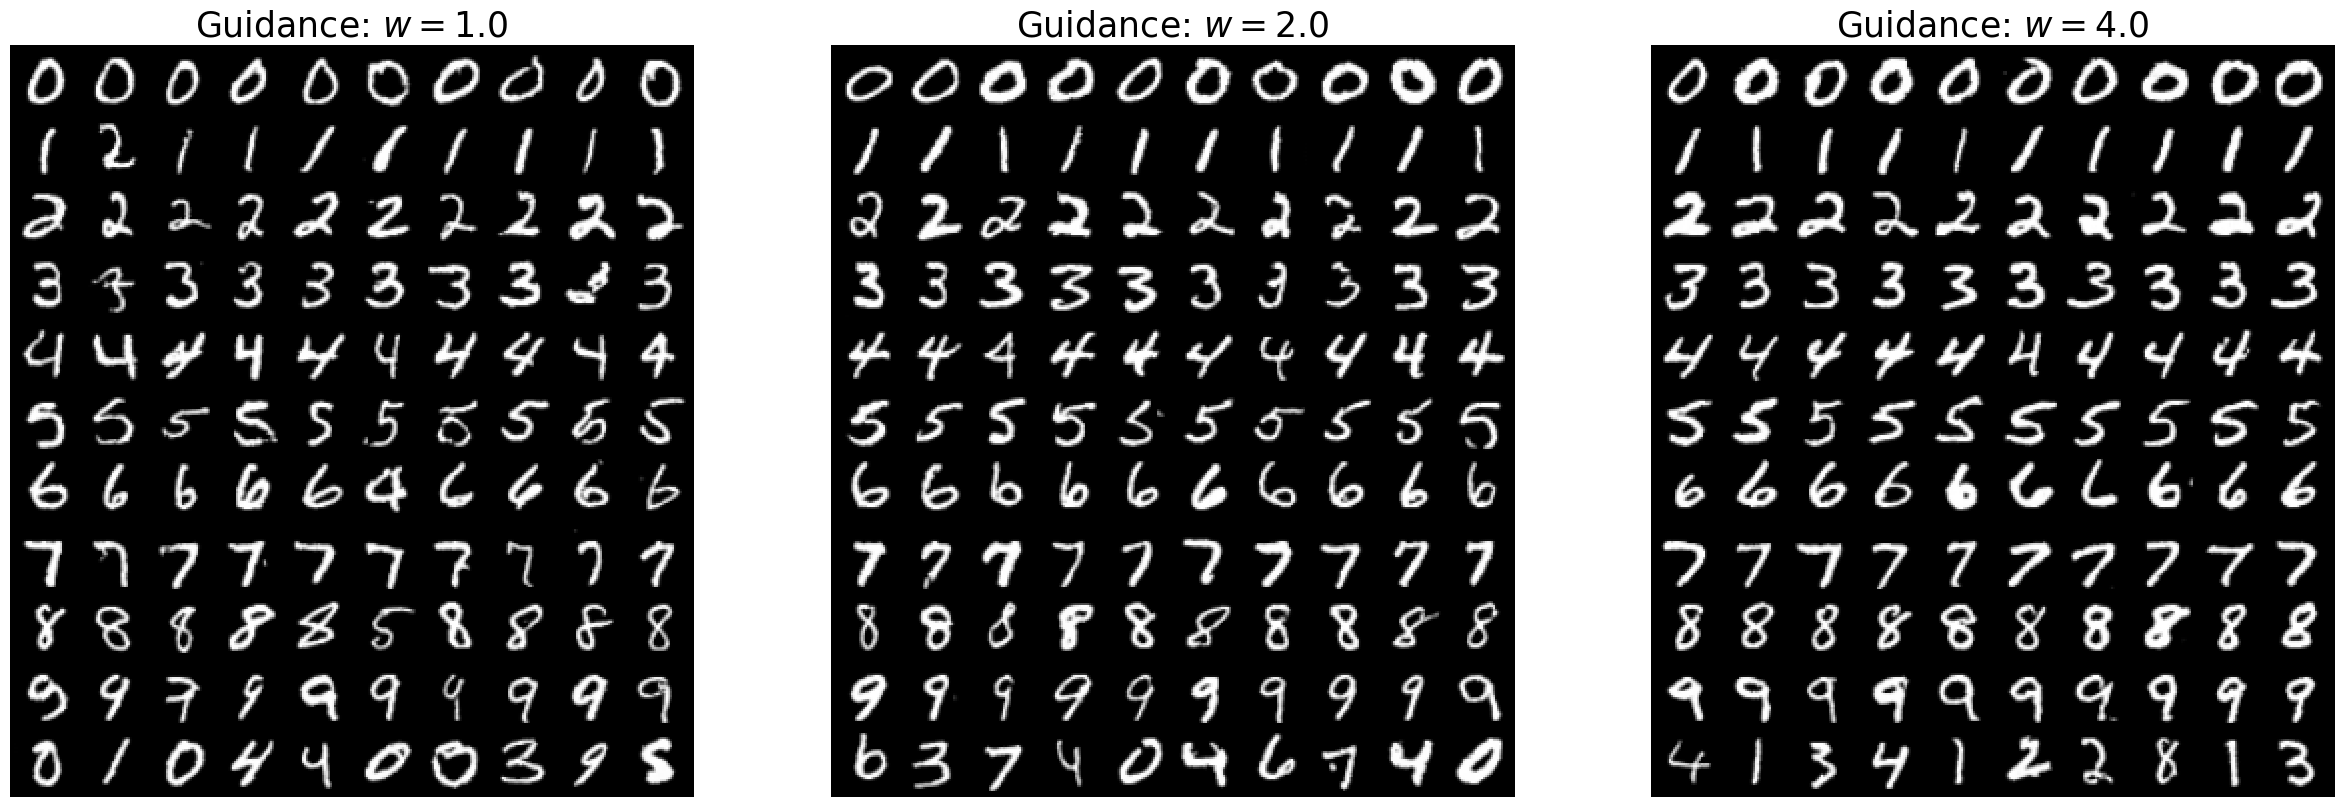
\includegraphics[width=0.82\linewidth]{tex/figures/selected/figure13-mnist-cfg.png}
  \caption{不同 guidance scale 下的 classifier-free guidance 效果。随着 $w$ 增大，样本通常更贴合条件，但多样性可能下降。}
  \label{fig:mnist-cfg-scale}
\end{figure}

图~\ref{fig:mnist-cfg-scale} 展示了 guidance scale 的典型影响：较大的 $w$ 会强化条件一致性，但也可能使样本更集中。
